\section{Automatic Code Optimization}\label{sec:aco:autosched}

    Automatic code optimization is a set of techniques implemented at the compiler level to automate time-consuming and expertise-demanding code optimization tasks typically done manually. The machine learning-based efforts made to achieve this goal can be classified, as outlined in the taxonomy in ~\Cref{sec:aco:autosched:taxonomy}. Further elaboration on this classification will be provided throughout this section.

    \begin{figure}[hbt!]
        \begin{center}
        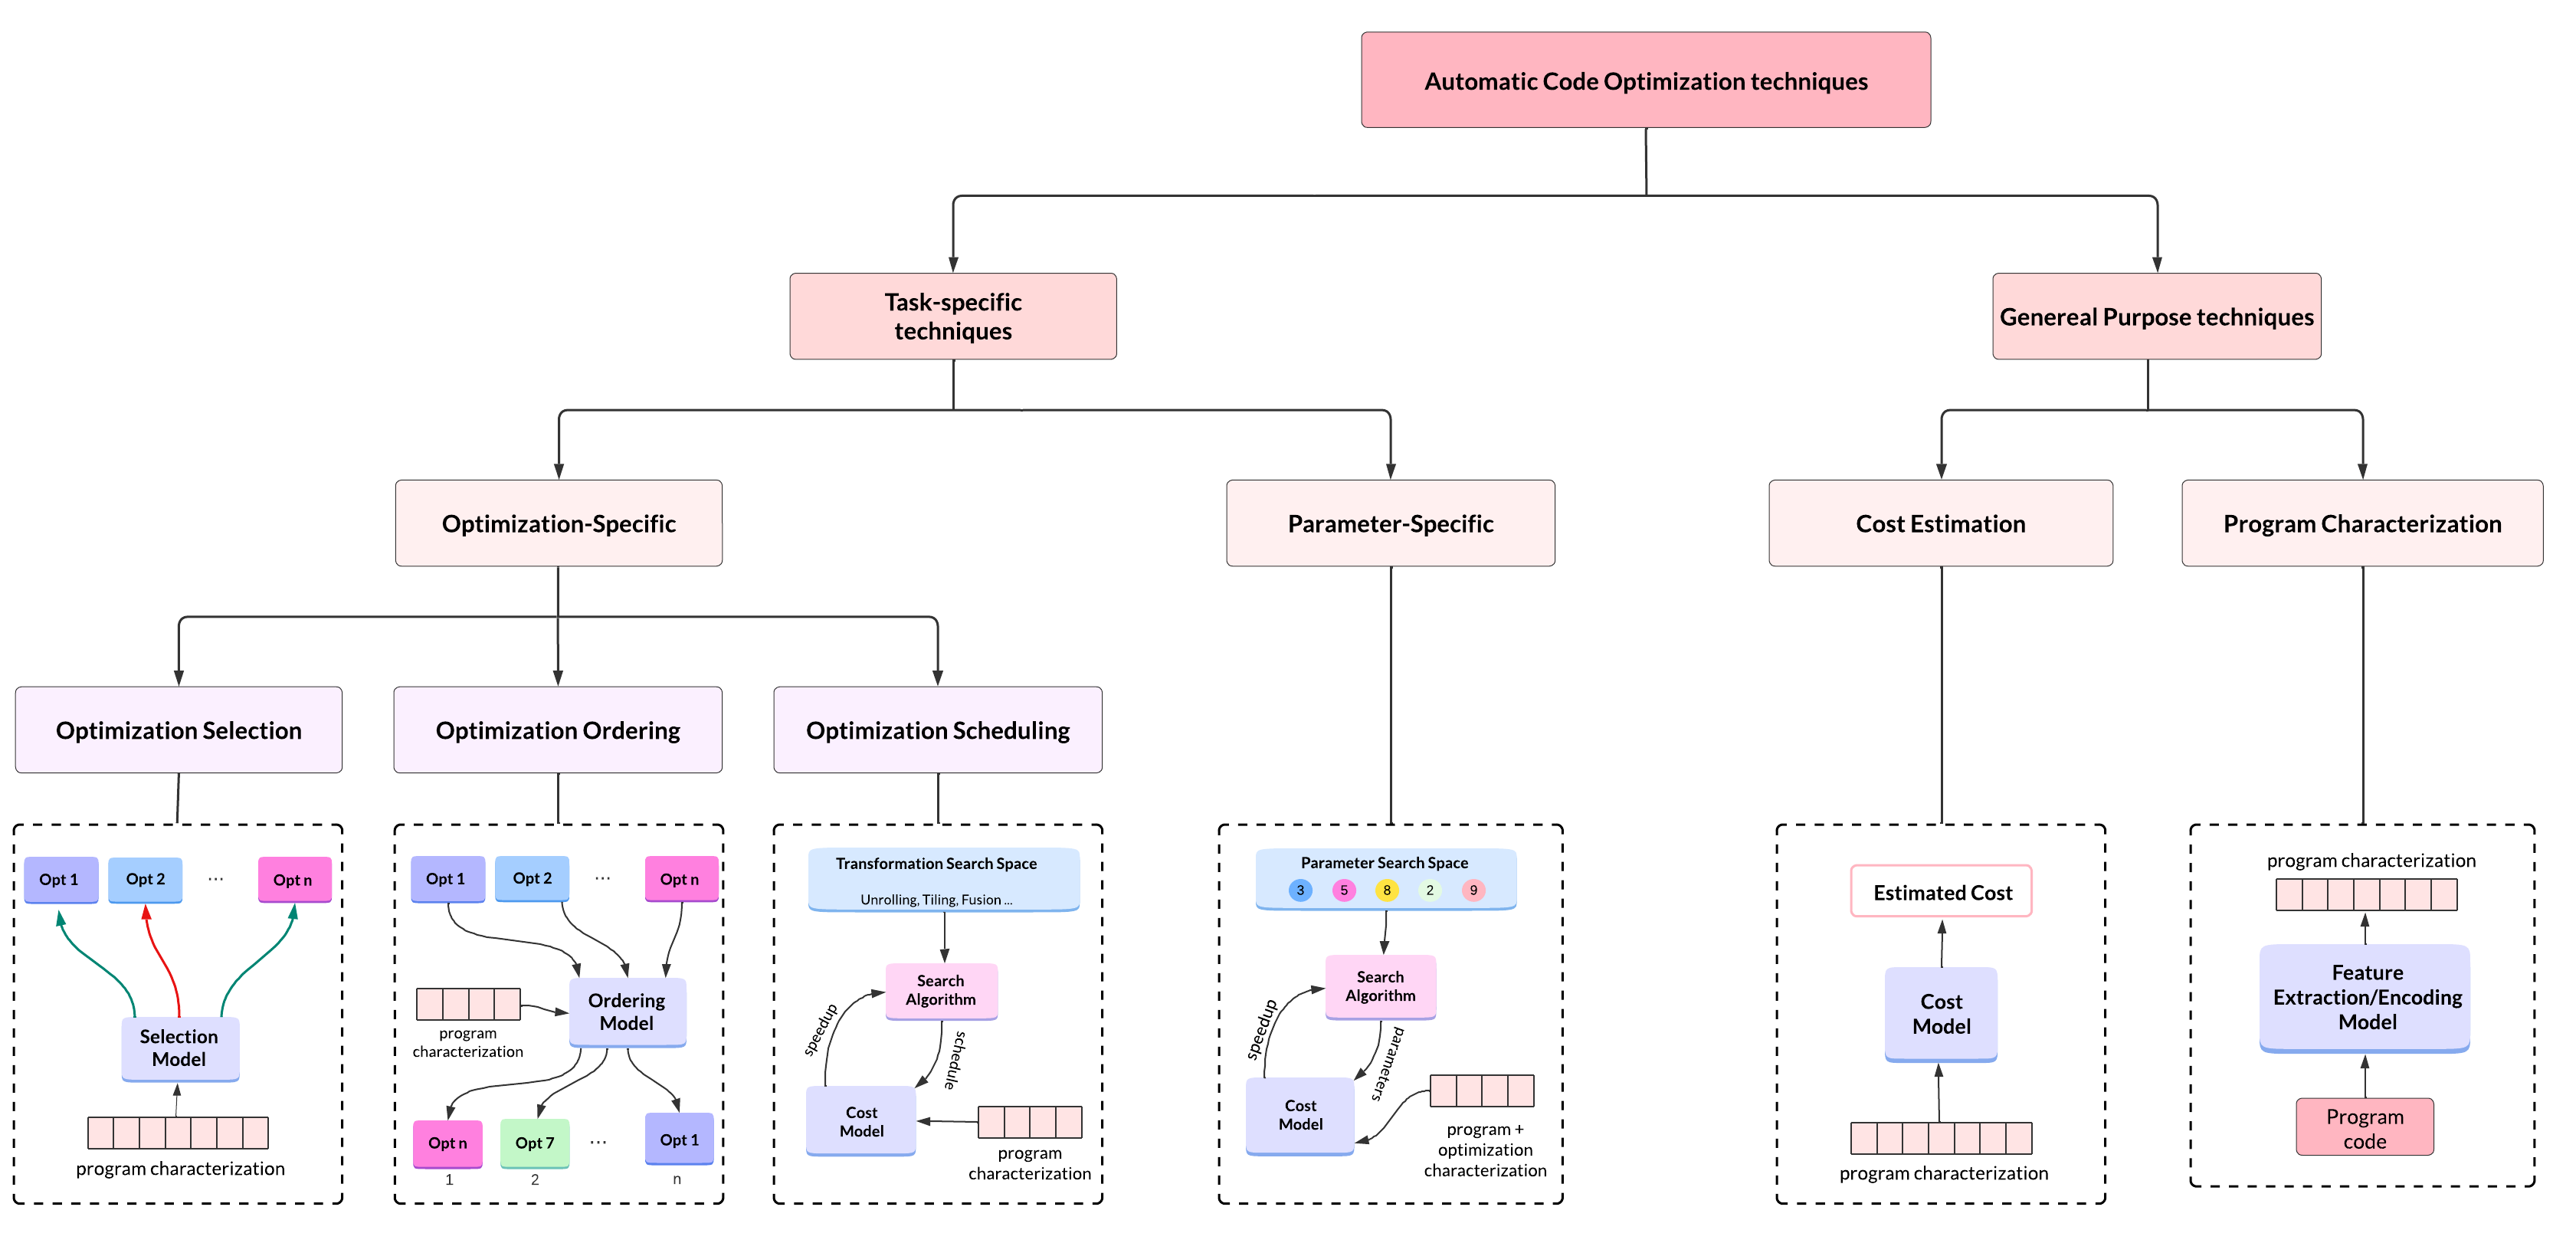
\includegraphics[width=1\textwidth]{assets/images/aco-taxonomy.png}
        \end{center}
        \caption{Automatic Code Optimization Techniques Taxonomy}%
        \label{sec:aco:autosched:taxonomy}
    \end{figure}

    
    \subsection{Task-Specific Techniques}

        Within this category, optimization techniques concentrate on addressing a particular code optimization task. This can be accomplished by intervening on the optimizations themselves or on their parameters.

        \subsubsection{2.3.1.1   Optimization-Level Techniques}
            On this level, automatic code optimization techniques engage directly with the optimizations rather than their parameters. This involvement can take various forms, such as selecting a specific set of optimizations to apply from a predetermined collection, determining the sequence in which a given set of optimizations is applied, or searching for the most effective sequence of applicable code optimizations within a designated transformation search space.
            
        
            \paragraph{Optimization Selection}
                Given a predefined set of code optimizations and transformation passes, selection techniques work on selecting which of them to apply. For example, in Milepost GCC~\cite{milepost}, which is a \gls{abb:ml}-based compiler, a 1-nearest-neighbor model is used to select the optimization flags to activate from a pool of approximately 100 flags available in GCC. The selection is based on hand-engineered features that represent the characteristics of the program.
            
            \paragraph{Optimization Ordering}
                The performance of a compiler-generated code depends on the order in which the optimization passes are applied~\cite{autophase}. Choosing a good application order for the optimization passes is often referred to as the phase ordering problem. 
                
                Autophase~\cite{autophase} tackles this problem on the LLVM compiler using deep \gls{abb:rl}. For that, 56 static features are extracted from LLVM programs \gls{abb:ir} (e.g., thenumber of blocks, branches, and instructions). The \gls{abb:rl} states are represented using these features. The performance metric is the number of clock cycles , and the used \gls{abb:rl} algorithms are Policy Gradient (PG) and Deep Q -Network (DQN).

                Another optimization ordering example is determine an ordering of nodes to consider when applying the fusion pass to fuse operations in a dataflow graph. In this context, ~\cite{fuse} proposed a priority-based operation fusion with an end-to-end deep \gls{abb:rl} model.
                The proposed network consists of a \gls{abb:gnn} that encodes the input graph into a vector representation. This \gls{abb:gnn} is jointly trained with the policy network that generates priorities, using a Proximal Policy Optimization (PPO)~\cite{ppo} algorithm. The framework architecture is illustrated in~\Cref{sec:aco:autosched:fuse}.

                \begin{figure}[hbt!]
                    \begin{center}
                    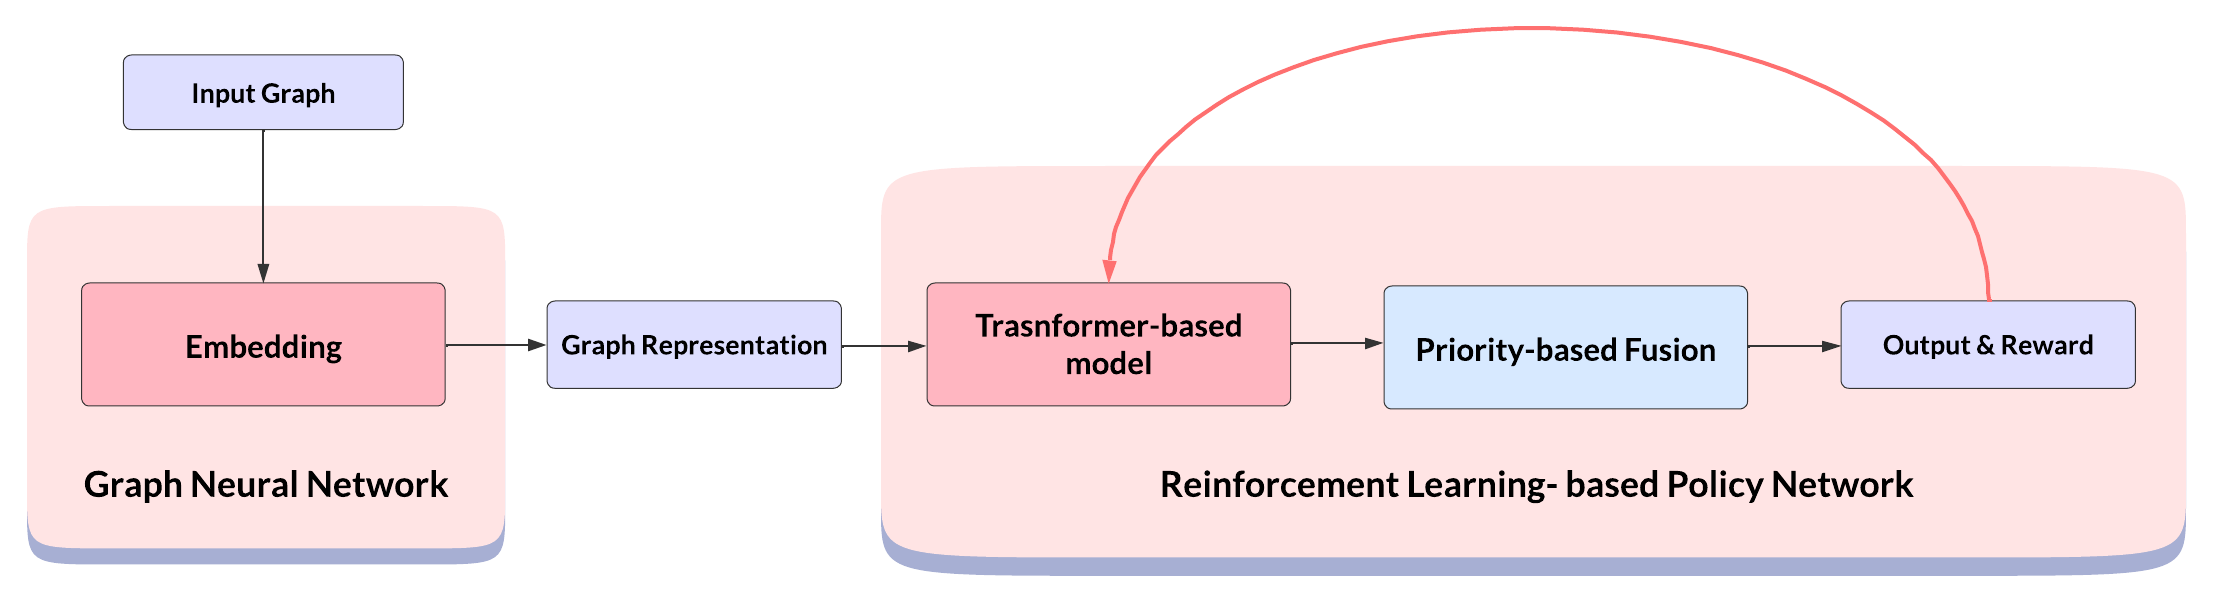
\includegraphics[width=.9\textwidth]{assets/images/fuse.png}
                    \end{center}
                    \caption{Learning to Fuse~\cite{fuse}}%
                    \label{sec:aco:autosched:fuse}
                \end{figure}

                

            
            \paragraph{Optimization Scheduling}
                
                Automatic optimization scheduling techniques, also known as autoscheduling techniques, involve the exploration of optimal schedules to achieve the maximum speedup for a given program. A schedule, defined as a sequence of code transformations (as discussed in the previous section), is typically searched within a designated search space by an algorithm that is guided by a cost model. This model evaluates candidate schedules by measuring the speedup they yield.

                Several notable works proposing autoscheduling techniques include the Halide autoscheduler~\cite{halide}, Tiramisu autoscheduler~\cite{tiramisu-autosched}, and Pluto~\cite{pluto}, which will be followingly introduced.

                Halide~\cite{halide} is a C++ embedded programming language designed for writing high-performance image and array processing code on modern machines. It provides an API to manually schedule algorithms within the same program. Additionally, Halide features an autoscheduler~\cite{halide} that automatically searches for the optimal schedule to apply to the program. The search space includes parallelization, loop unrolling, interchange, fusion, tiling and more code transformations (refer to the previous section). The exploration of this transformation space is done using Beam Search, guided by a \gls{abb:dnn}-based cost model that predicts the speedup achieved by a given candidate schedule. The model is a regression \gls{abb:ffnn} that takes in 54 manually engineering features that represent both algorithm-dependent and schedule-specific information and outputs the predicted speedup.

                On the other hand, Tiramisu ~\cite{tiramisu} is a \gls{abb:dsl} embedded in C++ that provides an \gls{abb:api} for writing high-level, architecture-independent code. It also provides a set of  \gls{abb:api} calls to perform code transformations on the written program. To automate finding the optimal sequence of transfomrations to apply, an autoscheduler has been implemented for Tiramisu~\cite{tiramisu-autosched}. The autoscheduler searches for the optimal sequence of loop trasnformations to apply on a given program to get the best speedup. The search has been conducted using both Beam Search and \gls{abb:mcts}, leveraging a cost model as a fitness function estimator to navigate the space. The cost model is a regression model that,  given features representing the unoptimized code and a sequence of code transformations,  predicts the speedup that we’d get from applying these transformations on the program. The model doesn’t rely on complex hand-engineered features, as it implements a mechanism for characterizing programs by extracting simple high-level information that is stored in a compact variable-size representation. This representation is based on the program’s \gls{abb:ast}, and it is in the form of an ordered tree of computation vectors. A computation vector includes loop nest representations, assignments and memory access representations and loop transformations representation. This representation is fed to the cost model, which has an architecture of three layers : a computation embedding layer that embeds each computation vector, a recursive loop embedding layer that recursively processes the resulting computation embeddings following the tree structure of the program,  and finally a regression layer that uses the resulting program embedding to predict the speedup.

                
            
            
        \subsubsection{2.3.1.2   Parameter-Level Techniques}
            Code transformations generally have one or more parameters to tune. A good parameter choice is crucial to take advantage of applying the transformation and yielding the wanted results. In this level, given a code transformation, optimization techniques will work on finding the optimal parameter configuration for that transformation.
            
            For instance, ~\cite{nntile} proposed a \gls{abb:nn} assisted search technique that searches for the best tile sizes given a program. The method computes the performance distribution based on a first random sampling phase, for which each randomly selected candidate tile size in the search space is empirically evaluated. Then, instead of randomly evaluating more points, the performance distribution is used to isolate a fraction of the space where the best tile sizes are predicted to be good.  For the performance estimation model, they use a fully connected \gls{abb:ffnn} that predicts the execution time given a tile size configuration. The network consists of an input layer with three input parameters (the tile sizes: Ti,Tj, Tk), an output layer with one output parameter (predicted execution time), and one hidden layer consisting of 30 hidden neurons.  The tile size configuration is presented as a three dimensional vector (Ti,Tj, Tk) representing the tile sizes of the three levels of nested loops that are being tiled. 
            
            Another example is AutoTVM~\cite{autotvm}. It is a compiler infrastructure tool implemented for the TVM compiler that uses simulated annealing to search the parameter space, and leavarages a \gls{abb:dnn} model to rank program versions with different transformation parameters, which significantly optimizes tensor programs. 
            For the model architecture, they proposed two types of models: the first is a statistical model, and the second is a \gls{abb:rnn}. The first model is based on gradient trees using domain-specific features of an \gls{abb:ast} such as memory access count, data reuse rate, etc. The second model is based on a TreeGRU~\cite{treegru}, which utilizes \gls{abb:ast} encoding to obtain a vector representation that passes through a linear layer for prediction.
        

    \subsection{General Purpose Techniques}

        \subsubsection{2.3.2.1   Cost Estimation Techniques}
            Many automatic code optimization tasks, like learning-based register allocation and instruction scheduling, rely on accurate cost estimations. However, executing code blocks at each optimization iteration is very costly. In this context, many cost estimation models has been proposed to be leveraged by techniques tackling these tasks. 
            
            For instance, Ithemal~\cite{ithemal} (Instruction THroughput Estimator using MAchine Learning) is a compiler infrastructure tool that predicts the throughput of a basic block in assembly-level, i.e. the number of clock cycles a processor takes to execute the block, based on the operation codes and operands of its instructions. It models the estimation problem as a regression task and solves it using a hierarchical LSTM trained on a large corpus of labeled data, mapping assembly sequences to real valued throughputs. Ithemal is fast, accurate and portable across a varierty of processor microarchitectures. However, it doesn't support high-level loop transformations and assumes that data is always in cache.

        \subsubsection{2.3.2.2   Program Characterization Techniques}
            \gls{abb:ml}-based code optimization techniques have been showing great results at automatically dealing with the complexity and diversity of modern hardware and software. However, their success is tighlty bounded by the quality of the features used to characterize programs. Features are usually manually engineered, which  makes the quality of the final model directly dependent on the skill and available time of the system architect.

            For this reason, it is necessary to find ways to design optimization techniques that automatically extract the program’s features that are the most relevant to the optimization task at hand.
            
            In this context, Deeptune~\cite{deeptune} has been proposed to faciliate the optimization of raw code by learning the embedding according to the chosen optimization task. This technique works by merging feature and heuristic construction into a single process of joint learning. It uses a pre-trained language model to constructs appropriate representations of the input code with respect to the optimization task, that is also learned at the same time by a \gls{abb:ffnn} connected to the output of the language model, as illustrated in~\Cref{sec:aco:autosched:deeptune}.

            \begin{figure}[hbt!]
                \begin{center}
                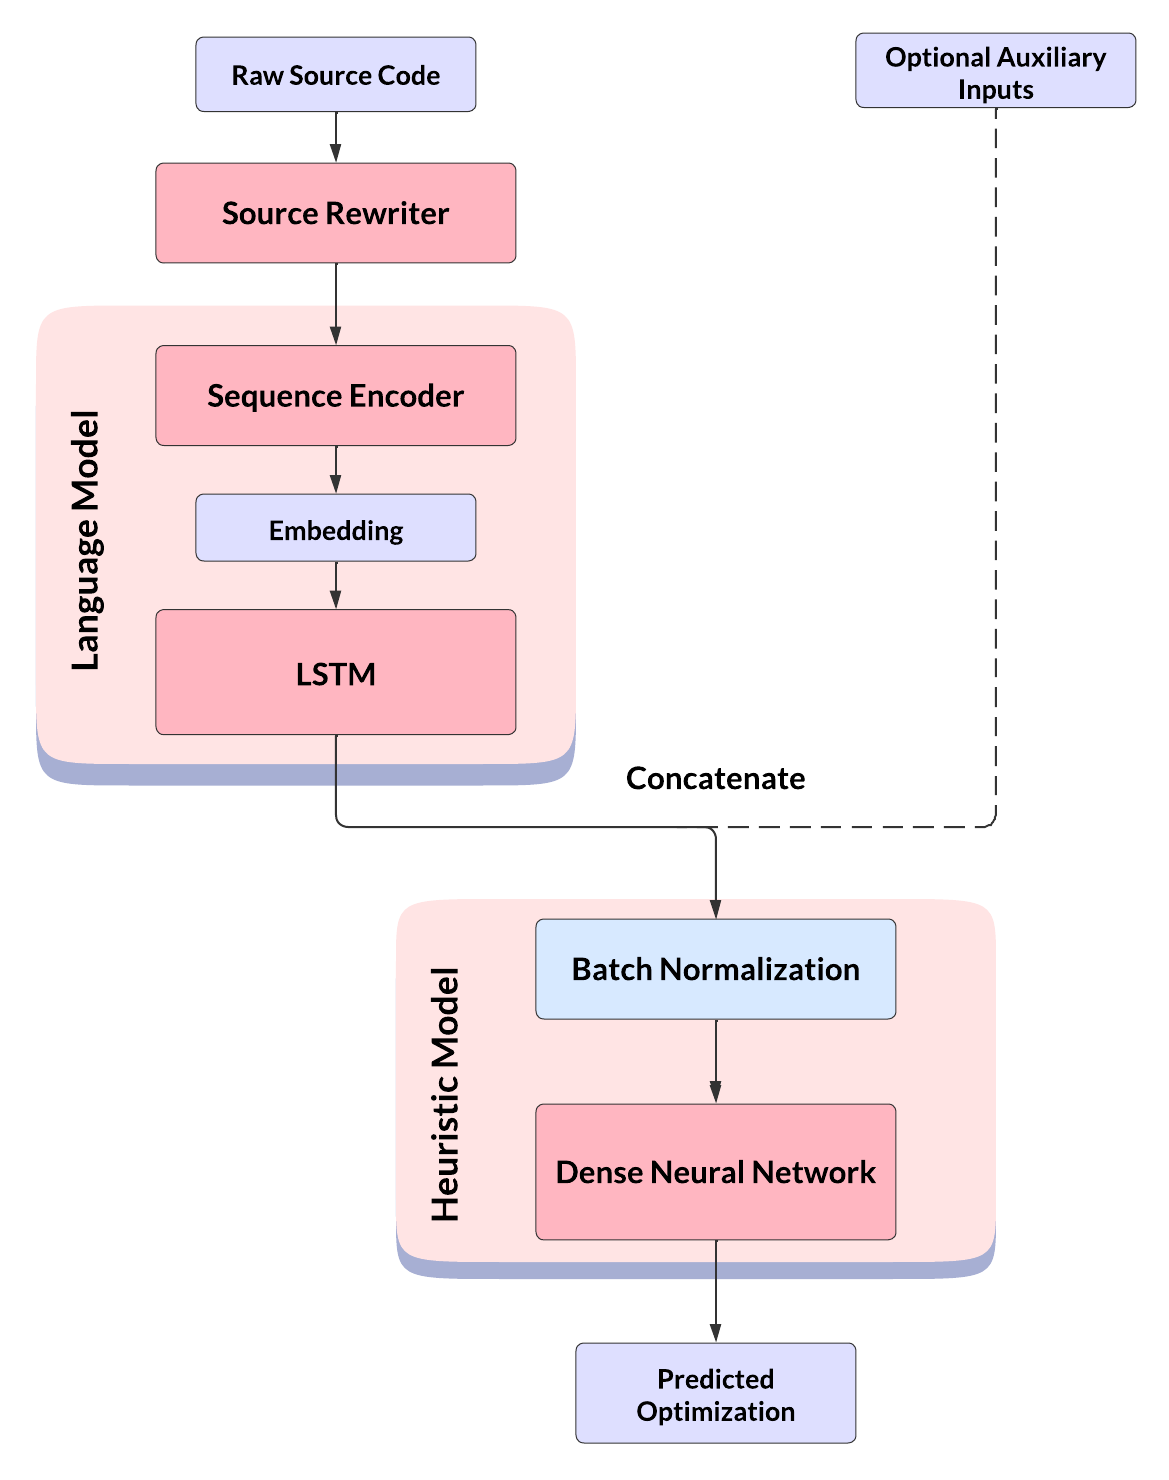
\includegraphics[width=.5\textwidth]{assets/images/deeptune.png}
                \end{center}
                \caption{Deeptune Model Architecture}%
                \label{sec:aco:autosched:deeptune}
            \end{figure}

